%! TEX root = course_report.tex

\section{Архитектура мобильного приложения} % (fold)
\label{sec:arch}


\subsection{Общая структура приложения}
\label{sub:arch:struct}

Исходный код приложения распределён по следующим папкам:
\begin{itemize}
	\item модуль данных (папка data);
	\item модуль внедрения зависимостей (папка di);
	\item модуль пользовательского интерфейса (папка ui);
	\item вспомогательные классы и функции (папка util).
\end{itemize}

Папка data содержит несколько подпапок:
\begin{itemize}
	\item database -- работа с базой данных SQLite;
	\item entity -- сущности для хранения в базе данных;
	\item file -- работа с файлами;
	\item model -- бизнес-логика приложения;
	\item service -- подключение по Bluetooth и др.
\end{itemize}

Директория ui включает в себя следующие поддиректории:
\begin{itemize}
	\item activity -- экраны (активности) приложения;
	\item adapter -- адаптеры для работы с RecyclerView;
	\item presenter -- логика отображения;
	\item util -- вспомогательные классы;
	\item view -- представления (наследники класса View);
	\item viewmodel -- модели представлений.
\end{itemize}

В приложении применён шаблон проектирования Model-View-ViewModel. Он используется для разделения модели и её представления, что необходимо для их изменения отдельно друг от друга. Например, разработчик задаёт логику работы с данными, а дизайнер работает с интерфейсом. Шаблон проектирования MVVM является одним из представителей группы Model-View-Controller, но содержит некоторые отличия от стандартного MVC.

MVVM удобно использовать вместо классического MVC и ему подобных в тех случаях, когда в платформе, на которой ведётся разработка, есть «связывание данных».
В шаблонах проектирования MVC/MVP изменения в пользовательском интерфейсе не влияют непосредственно на Mодель, а предварительно идут через Контроллер (англ. Controller) или Presenter.
В таких технологиях, как Android, есть концепция «связывания данных», позволяющая связывать данные с визуальными элементами в обе стороны.
Следовательно, при использовании этого приёма применение модели MVC становится крайне неудобным из-за того, что привязка данных к представлению напрямую не укладывается в концепцию MVC/MVP \cite{android_view_model}.

\subsection{UML-диаграмма приложения}
\label{sub:arch:struct}

Диаграмма классов (англ. class diagram) — структурная диаграмма языка моделирования UML, демонстрирующая общую структуру иерархии классов системы, их коопераций, атрибутов (полей), методов, интерфейсов и взаимосвязей между ними. Широко применяется не только для документирования и визуализации, но также для конструирования посредством прямого или обратного проектирования.
Целью создания диаграммы классов является графическое представление статической структуры декларативных элементов системы (классов, типов и т. п.) Она содержит в себе также некоторые элементы поведения (например, операции), однако их динамика должна быть отражена на диаграммах других видов (диаграммах коммуникации, диаграммах состояний). Для удобства восприятия диаграмму классов можно также дополнить представлением пакетов.

На рисунке \ref{fig:uml_diagram} изображён фрагмент UML-диаграммы классов.

\begin{figure}[ht]
    \centering
    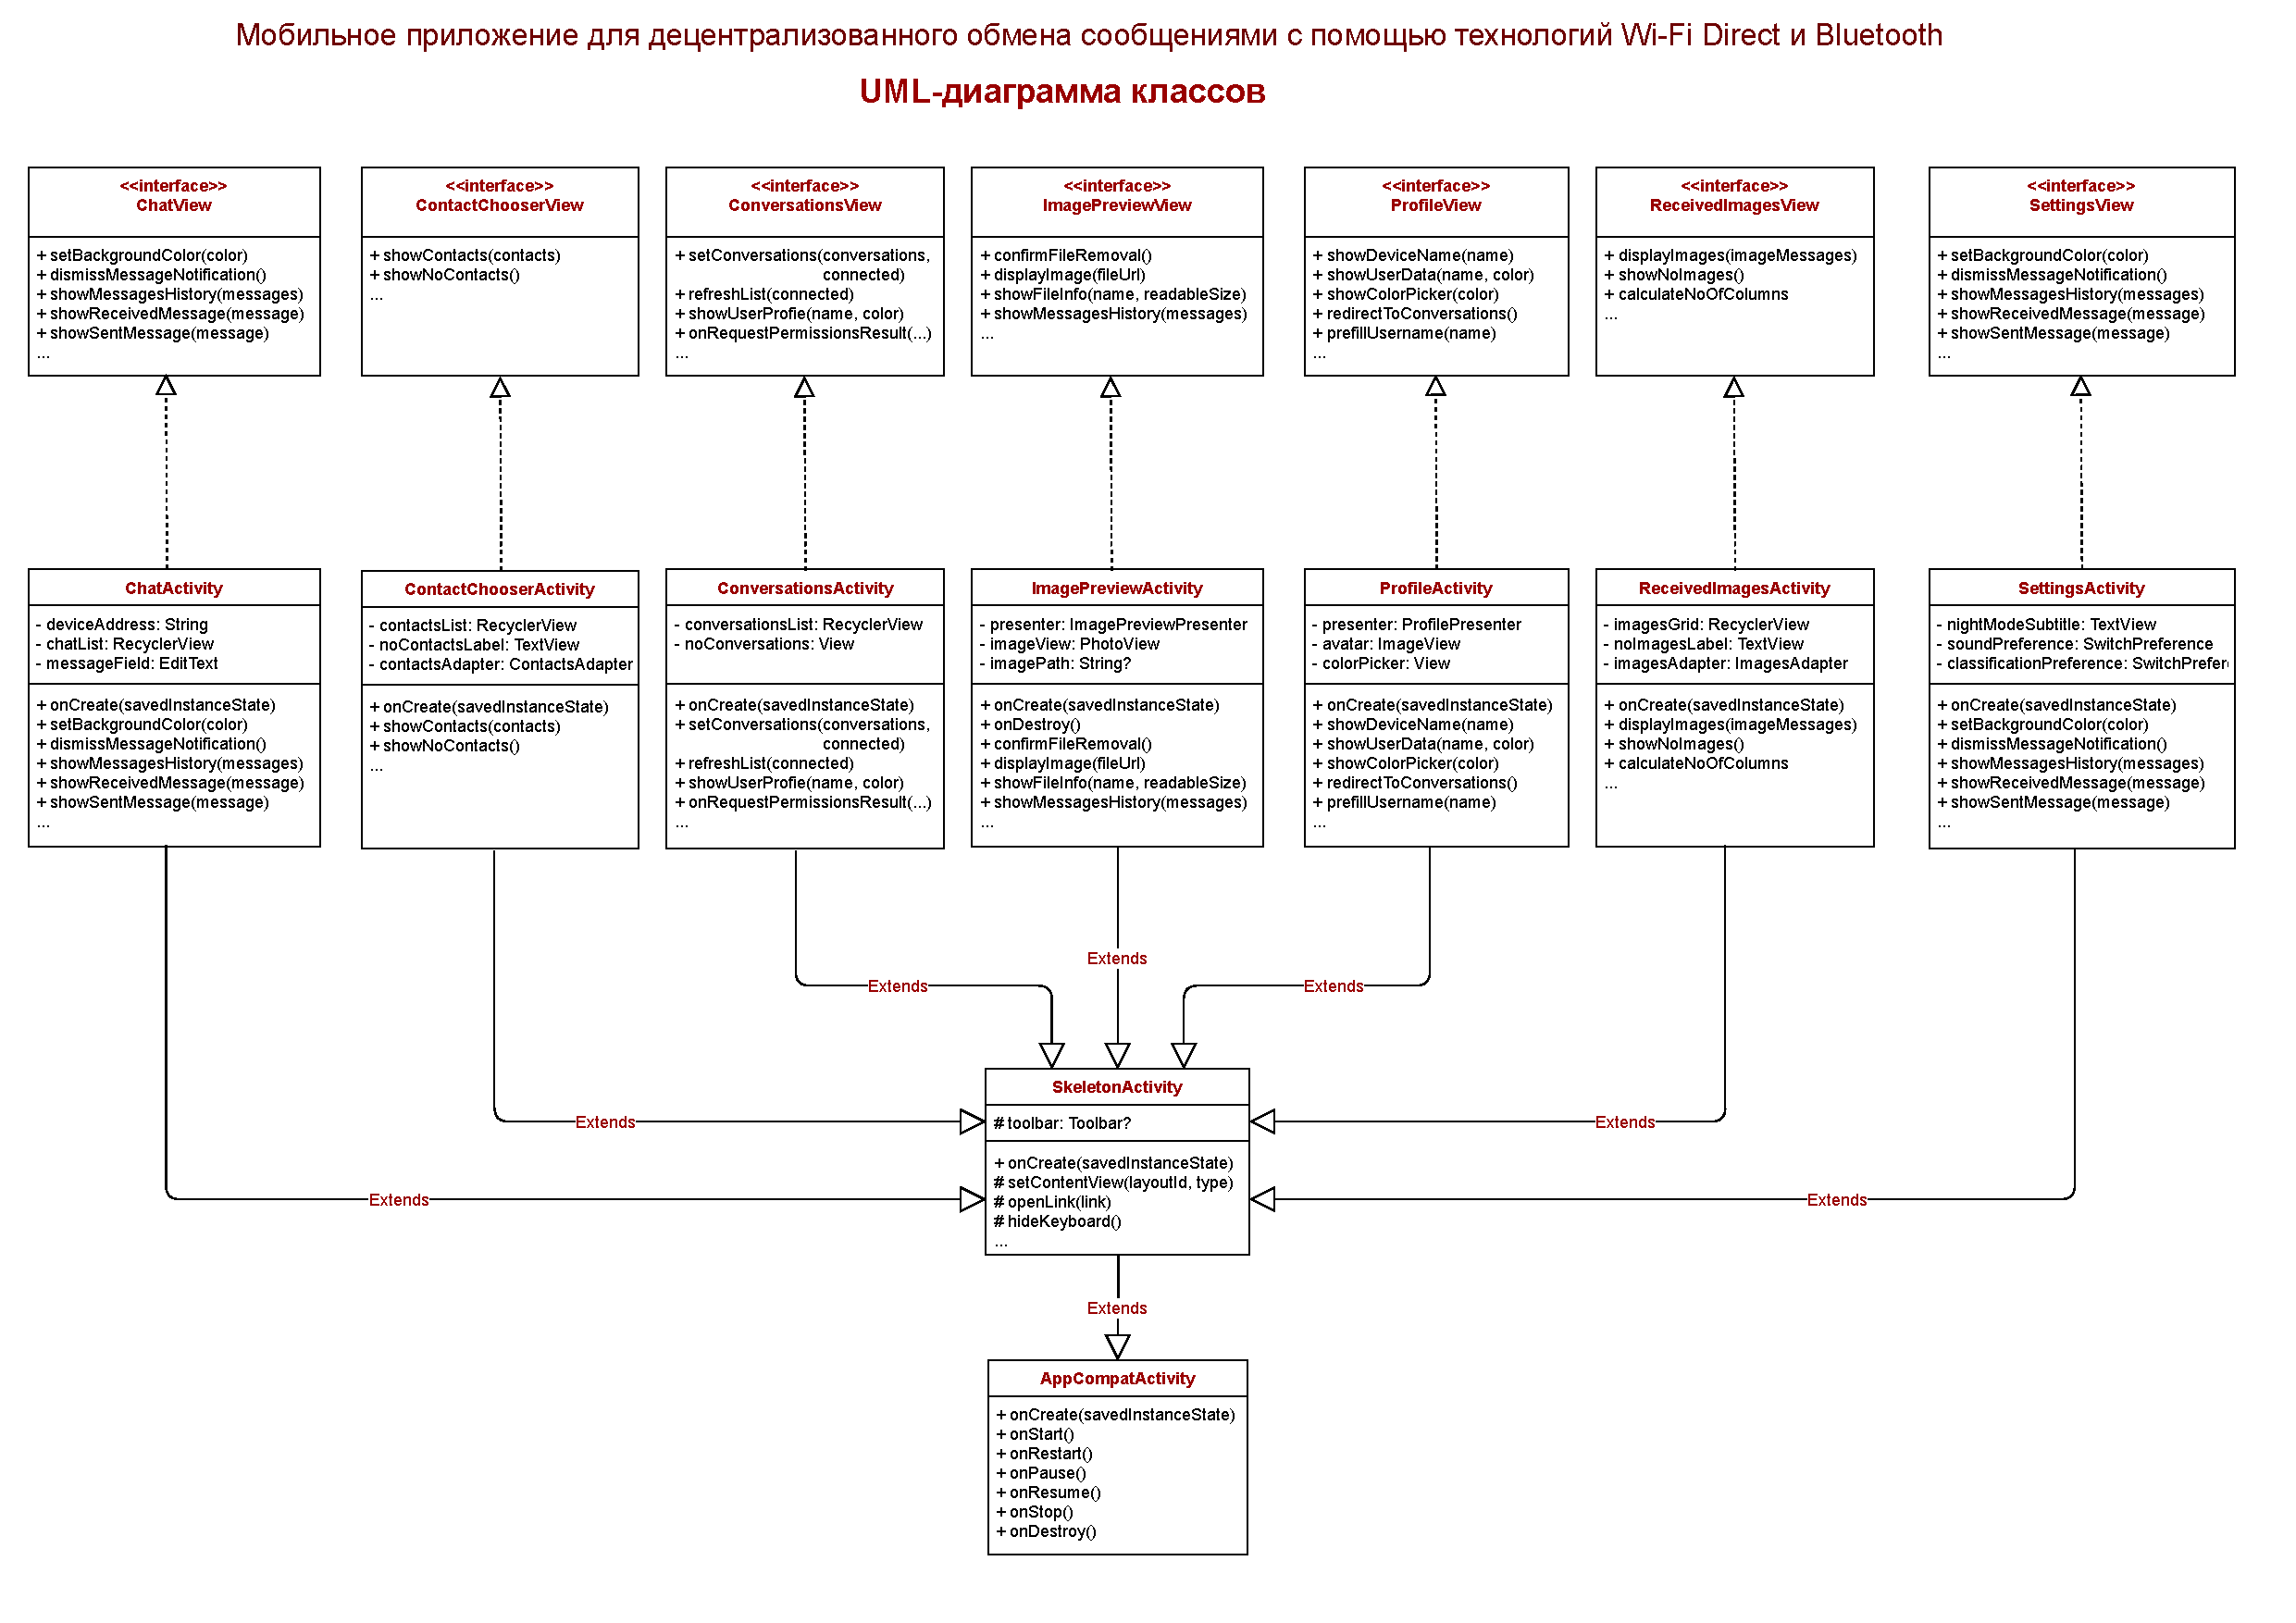
\includegraphics[width=1.0\textwidth]{class_diagram.pdf}
    \caption{Фрагмент UML-диаграммы классов разработанного приложения}
	\label{fig:uml_diagram}
\end{figure}

Данная диаграмма описывает отношения наследования между классами отображения интерфейса из групп Activity и View.

\subsection{Конфигурация Gradle и используемые библиотеки}
\label{sub:arch:deps}

Для сборки исходного кода приложения была использована система сборки Gradle.
Конфигурация Gradle для данного проекта хранится в файлах build.gradle.kts, settings.gradle.kts, gradle.properties, а также app/build.gradle.kts. Файлы конфигурации Gradle с расширением .kts написаны на специальном подмножестве языка программирования Kotlin.

В файле build.gradle.kts содержится информация об используемых репозиториях. В частности, в данном проекте подключены использованы следующие репозитории библиотек:
\begin{itemize}
	\item Google -- компоненты AndroidX и др.;
	\item Jcenter;
	\item Fabric.io;
	\item Maven Central (Gradle обратно совместим с артефактами Maven);
	\item Maven Bintray;
	\item JitPack -- позволяет подключать GitHub репозитории одной строкой;
	\item SonaType.
\end{itemize}

Кроме репозиториев, build.gradle.kts содержит версию Android Gradle плагина, а также плагина Kotlin.

Файл app/build.gradle.kts описывает версии библиотек, используемые в приложении. Разработанное приложение использует довольно большое количество библиотек, среди них:
\begin{itemize}
	\item androidx.appcompat:appcompat -- обратная совместимость с устаревшими версиями платформы Android;
	\item androidx.recyclerview:recyclerview -- компонент для отображения прокручиваемого списка элементов с динамической загрузкой;
    \item androidx.cardview:cardview -- компонент для карточек в стиле Material;
    \item androidx.constraintlayout:constraintlayout -- поддержка ConstraintLayout;
    \item com.google.android.material:material -- поддержка Material Design, разработанного компанией Google в 2014 г.
    \item androidx.room:room-runtime -- более удобный интерфейс для работы с базой данных SQLite, используемой в платформе Android по умолчанию.
    \item room:room-compiler -- плагин компилятора для поддержки аннотаций, используемых библиотекой Room;
	\item androidx.lifecycle:lifecycle-runtime -- среда времени выполнения для удобной работы с жизненным циклом приложения (lifetime);
    \item androidx.lifecycle:lifecycle-extensions -- плагин компилятора для поддержки специальных аннотаций Android LifeCycle;
    \item lifecycle:lifecycle-compiler -- плагин компилятора для LifeCycle;
	\item com.timehop.stickyheadersrecyclerview:library -- RecyclerView с неподвижным заголовком (<<липким>>);
    \item com.amulyakhare:com.amulyakhare.textdrawable -- компонент для рисования текста на элементе типа Drawable, использован в приложении для генерации аватарок с буквами имени;
    \item com.github.chrisbanes:PhotoView -- библиотека для просмотра фото;
    \item com.squareup.picasso:picasso -- библиотека для передачи и загрузки изображений, предназначенная для использования с Android;
    \item com.github.jkwiecien:EasyImage -- ещё одна библиотека;
    \item me.priyesh:chroma -- меню выбора цвета в стиле Material Design;
    \item org.koin:koin-android -- фреймворк инъекции зависимостей;
	\item org.jetbrains.kotlin:kotlin-stdlib-jdk8 -- стандартная библиотека языка программирования Kotlin, совместимая с Java 8 (работает и на Java 11);
    \item org.jetbrains.kotlinx:kotlinx-coroutines-core -- поддержка корутин для языка программирования Kotlin;
    \item org.jetbrains.kotlinx:kotlinx-coroutines-android -- поддержка корутин для языка программирования Kotlin в контексте платформы Android;
    \item com.github.joshjdevl.libsodiumjni:libsodium-jni-aar -- библиотека криптографических функций
\end{itemize}

Ключевым компонентом для создания визуального интерфейса в приложении Android является activity (активность). Нередко activity ассоциируется с отдельным экраном или окном приложения, а переключение между окнами будет происходить как перемещение от одной activity к другой. Приложение может иметь одну или несколько activity. Например, при создании проекта с пустой Activity в проект по умолчанию добавляется один класс Activity - MainActivity, с которого и начинается работа приложения

Жизненный цикл в Android -- набор состояний Activity и переходов между ними (конечный автомат). На рисунке \ref{fig:lifecycle} показан жизненный цикл Activity.

\clearpage

\begin{figure}[ht]
    \centering
    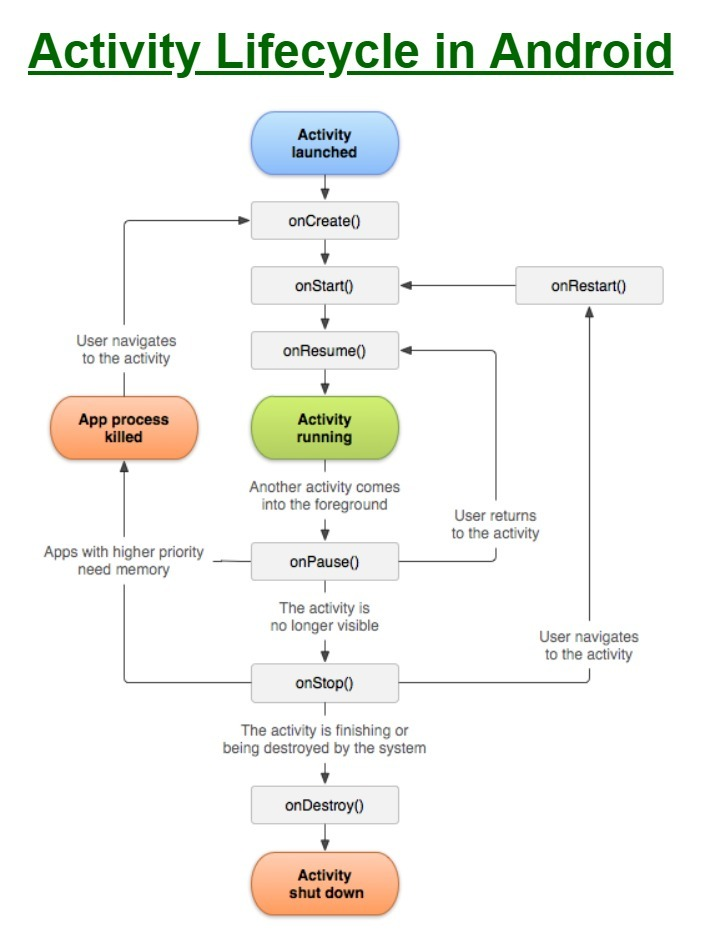
\includegraphics[width=0.8\textwidth]{lifecycle.jpg}
	\caption{Жизненный цикл Activity}
	\label{fig:lifecycle}
\end{figure}

Все объекты activity представляют собой объекты класса Activity, которая содержит базовую функциональность для всех activity.
На практике напрямую с этим классом не работают.
MainActivity наследуется от класса AppCompatActivity.
Однако сам класс AppCompatActivity, хоть и не напрямую, наследуется от базового класса Activity.
